\subsection{Merkmalsextraktion} \label{merkmalsextraftion-1}


Wie bereits in Kapitel \ref{merkmalsextraktion-0} beschrieben, ist das Ziel der Merkmalsextraktion Charakteristiken und Merkmale in den Daten zu finden, die f{\"u}r das
Klassifizierungsproblem von m{\"o}glichst hoher Relevanz sind. Im Rahmen des ELISE Projektes haben wir verschiedene Vorgehensweisen angewendet. Im den folgenden Unterkapiteln werden diese vorgestellt. \\


% Unterkapitel 
\subsubsection{Handgefertigte Merkmale} \label{hc-features-1}
Der handgefertigten Merkmal Ansatz (enlg. "hand-crafted features approach") besteht in der Berechnung relativ einfacher Merkmale von denen vermudetet wird, dass sie f{\"u}r das Klassifizierungsproblem der Eingangssignale relevant sein k{\"o}nnen. Diese Vorgehensweise hat den Vorteil des einfachen Aufbaus als auch der relativ geringen ben{\"o}tigten Rechenleistung, wobei potentiell gute Klassifizierungsergebnisse erwarten werden. \\


Obwohl fr{\"u}here Forschungsarbeiten schon handgefertigte Merkmale zur Emotionserkennung unter mithilfe physiologischer Signale getestet haben (vgl. \cite{martinez_ieee_2013}), wurde dieser Ansatz noch nie f{\"u}r die Erkennung dieser spezifischen Emotionen unter Verwendung dieser Kombination von Sensoren getestet.
Zus{\"a}tzlich haben wir zuerst handgefertigte Merkmale getestet, um ein Basisergebnis zu liefern, mit der die Ergebnissen der anderen Ans{\"a}tze vergleichen werden k{\"o}nnen.
Handgefertigte Merkmale sind in der Regel entweder einfache statistische Werte, Fourier-basierte oder selbstentwickelte Merkmale sein, die aufgrund von Vorkenntnissen der Daten verwendet werden. 
Diese Arbeit wurden statistische, Fourier-basierte und selbstentwickelte Merkmale getestet. \\

\textbf{Statistische Merkmale \\}
Die Tabelle \ref{tab:statistische} fasst die elf verschiedenen und in der Studie verwendeten statistischen Merkmale zusammen \cite{bscpiet}. Wir bezeichnen $\mathbf{x} = (x_1, x_2, ...., x_T) $ als Vektor, der die in einem Datenzeitfenster der L{\"a}nge $T$ enthaltenen Sensorwerte f{\"u}r einen Sensorkanal darstellt. 


\begin{table}[h]
\begin{tabular}{| l | p{12.5cm} |}
\hline
    \textbf{Merkmalname}     &  \textbf{Definition}  \\ \hline
    
    Mittelwert         & \vspace{0.01cm}
    $ mean(\mathbf{x}) =$ \Large{$\frac{1}{T} \sum_{k=1}^T (x_k) $} \\[0.5cm] \hline 
    
    Standard-Abweichung        & \vspace{0.01cm}
    $ \sigma(\mathbf{x}) =$ \Large{$ \sqrt{ \frac{1}{T} \sum_{k=1}^{T}{(x_k - \mu)^{2}} } $ } \\[0.5cm] \hline
    
    Maximum                   & \vspace{0.01cm}
    $ max(\mathbf{x}) = \max(x_{1},x_{2},\dots ,x_{T}) $
    \\[0.5cm] \hline
    
    Minimum                   & \vspace{0.01cm}
    $ min(\mathbf{x}) = \min(x_{1},x_{2},\dots ,x_{T}) $
    \\[0.5cm] \hline
    
    Amplitude                 & \vspace{0.01cm}
    $ A(\mathbf{x}) = max(\mathbf{x}) - min(\mathbf{x}) $ 
    \\[0.5cm] \hline
    
    25/50/75\% Perzentil      & Wert einer Menge, unter dem 25/50/75\% der Werte aus der Menge fallen. \\ \hline
    
    Interquartiler Bereich    & Differenz zwischen dem 75. und 25. Perzentil.
    \\ \hline
     
    Schr{\"a}ge                   & \vspace{0.01cm}
    $ \gamma _{1}(\mathbf{x}) = \operatorname{E}$ \Large{$\left[\left({\frac {X-\mu }{\sigma }}\right)^{3}\right]$ \normalsize{$=$} ${\frac {\mu _{3}}{\sigma ^{3}}}$ \normalsize{$=$} ${\frac {\operatorname {E} \left[(X-\mu )^{3}\right]}{ (\operatorname {E} \left[(X-\mu )^{2}\right])^{3/2}}}$ \normalsize{$=$} ${\frac {\kappa _{3}}{\kappa _{2}^{3/2}}} $} \vspace{0.2cm}
    \\[0.3cm] \hline
     
    Kurtosis                  & \vspace{0.01cm}
    $ \operatorname {Kurt}[\mathbf{x}] = \operatorname{E} $ \Large{$\left[\left({\frac {X-\mu }{\sigma }}\right)^{4}\right]$ \normalsize{$=$} ${\frac {\mu _{4}}{\sigma ^{4}}}$ \normalsize{$=$} ${\frac {\operatorname {E} [(X-\mu )^{4}]}{(\operatorname {E} [(X-\mu )^{2}])^{2}}} $} \vspace{0.2cm}
    \\[0.3cm] \hline
\end{tabular} 
\caption[Statistische Merkmale]{Statistische Merkmale, die im Rahmen des ELISE-Projektes verwendet wurden. } \label{tab:statistische}
\end{table} 


\textbf{Fourier-basierte Merkmale \\}
Die in diesem Kapitel pr{\"a}sentierten Ergebnisse wurden in einer Bachelorarbeit \cite{bsclittau} ermittelt, die auch ihm Rahmen des ELISE-Projektes geschrieben wurde. \\

Die Transformation von Zeitsignalen im Frequenzbereich bei Studien zu einem g{\"a}ngigen Werkzeug f{\"u}r die Analyse von Zeitreihendaten geworden. Es basiert auf einem mathematischen Prozess namens Fouriertransform, wo ein Signal in einer unendlichen gewichteten Summe von Sinus- und Coisnewellen unterschiedlicher Frequenz zu zerlegen.
Bei einer kontinuierlichen Funktion $ f : t \rightarrow f(t) $ ist der Fouriertransformation $ F(w) $ eines Signals $ f $: 
\begin{equation} 
\Large{ F(w) = \int\limits_{-\infty}^{\infty}{f(t)e^{-2\pi{}iw}dt}} 
\label{equ:fourier} \end{equation}
\vspace{0.2cm}

In den meisten realen Anwendungen sind die Signale jedoch diskontinuierlich. 
Eine alternative Fourier-Transformation, die sogenannte diskrete Fourier-Transformation (engl. "discrete fourier transform"), kann dann stattdessen angewendet werden.
Ein diskretes Signal $ x = (x_{0},x_{1},x_{2},...,x_{N-1}) $ von N Punkten wird durch die folgende Formel gegeben:
\begin{equation} 
\Large{ X_{k} = \sum\limits_{n=0}^{N-1} x_{n} e^{- \frac{2 \pi i}{N} kn} } 
\end{equation} 
\vspace{0.2cm}

wobei die Koeffizienten $ X_{k} \in \mathbb{C} $ die Fourier-Koeffizienten des Originalsignals sind.
Die Fourier-Koeffizienten werden haupts{\"a}chlich verwendet, um das Leistungsspektrum (engl. "power spectrum") $ p(x) $ des Signals $x$ zu berechnen, das Auskunft {\"u}ber den Beitrag jeder Frequenzkomponente zum Signal gibt. 
Die Komponenten $ p_{k}(x) $ des Leistungsspektrums f{\"u}r $ k \in \lbrace 0,1,...,N-1 \rbrace$ werden berechnet durch: 
\begin{equation} 
\Large{ p_{k}(x) = \Re(X_{k}^{2})+\Im(X_{k}^{2}) } 
\end{equation} 

wobei $ p_{k}(x) $ mit der Energie des Singals $x$ verglichen werden kann, das der $k$-ten Frequenz zugeordnet ist. \\


Um frequenzbezogene Merkmale zu extrahieren, wird das Leistungsspektrum der Signale in vier Frequenzb{\"a}nder gleicher L{\"a}nge unterteilt.
Der Mittelwert, die Standard-Abweichung, das Maximum und das Minimum wurde dann auf jedem Frequenzband f{\"u}r jeden Sensorkanal extrahiert, was zu einem Prozess der Merkmalsextraktion aus normalisierten Datenrahmen f{\"u}hrte, wie in Abbildung \ref{fig:fft} dargestellt. 

\begin{figure}[h] \centering{
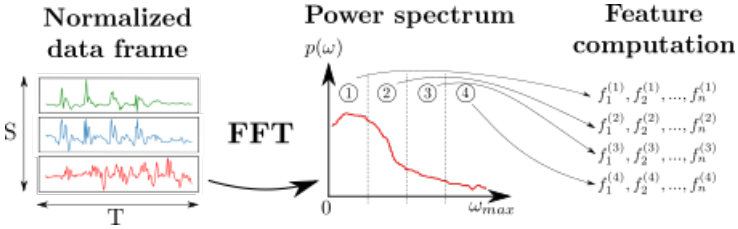
\includegraphics[width=11cm]{Images/ttf.png}}
\caption[Merkmalsextraktion aus frequenzbezogener Domain]{ Merkmalsextraktion aus frequenzbezogener Domain. } 
\label{fig:fft} \end{figure} \vspace{0.5cm}


Zus{\"a}tzlich wurde f{\"u}r jeden Sensorkanal des gesamten Spektrums die Standard-Abweichung  extrahiert. Dies f{\"u}hrt zu insgesamt $9 \ast (1 + 4 \ast 4) = 153$ Merkmalen im Frequenzbereich pro Zeitfenster. \\


\textbf{Selbstentwickelte Merkmale \\}
Es wurden zwei eigene Merkmale definiert \cite{bscpiet}. Nulldurchgang (engl. "zero crossing") und Anzahl der Spitzen (engl. "number of peaks"). Im Folgendem werden diese beiden Merkmale detailiert beschrieben. \\

Das Nulldurchgang-Merkmal z{\"a}hlt die H{\"a}ufigkeit, mit der das Signal eines Sensorkanals in einem Zeitfenster die Nulllinie {\"u}berschreitet.
Alle Sensorsignale wurden durch Normierung verarbeitet (vgl. Kapitel \ref{vorverarbeitung-1}) und damit wurden alle Mittelwerte auf Null zentriert.
Um zu vermeiden, dass Rauschen entlang der Nulllinie in dem Merkmal gez{\"a}hlt wird, wird nur ein Nulldurchgang in einer bestimmten Zeitspanne gez{\"a}hlt. \\


Das Spitzenz{\"a}hler-Merkmal bestimmt die Anzahl von loklanen Hochpunkten im Zeitsignal.
Alle lokalen Maximen sind durch einen Onset (Startpunkt), eine Spitze und einen Offset (Endpunkt) gekennzeichnet (vgl. Abbildung \ref{fig:peaks}). 
Jedes Vorkommen einer Onset/Offset-Paarung wird hierbei als Spitze gez{\"a}hlt.
Onsets, Spitzen und Offsets werden durch die folgenden Operationen identifiziert (vgl. \cite{bscGouverneur}):

\begin{itemize} %[noitemsep]
  \item Ein Onset wird bestimmt, wenn der Wert des Signals an diesem Punkt nicht negativ ist und die Differenz zwischen ihm und dem n{\"a}chsten gr{\"o}{\ss}er als ein vordefinierter Schwellenwert (engl. "threshold") ist.

  \item Ein Offset wird bestimmt, wenn der Wert des Signals kleiner als der Wert des zuletzt gesetzten Onsets ist.

  \item Das lokale Maximum zwischen einem Onset und Offset wird als Spitze bezeichnet.
\end{itemize} \vspace{0.2cm}


\begin{figure}[h] \centering{
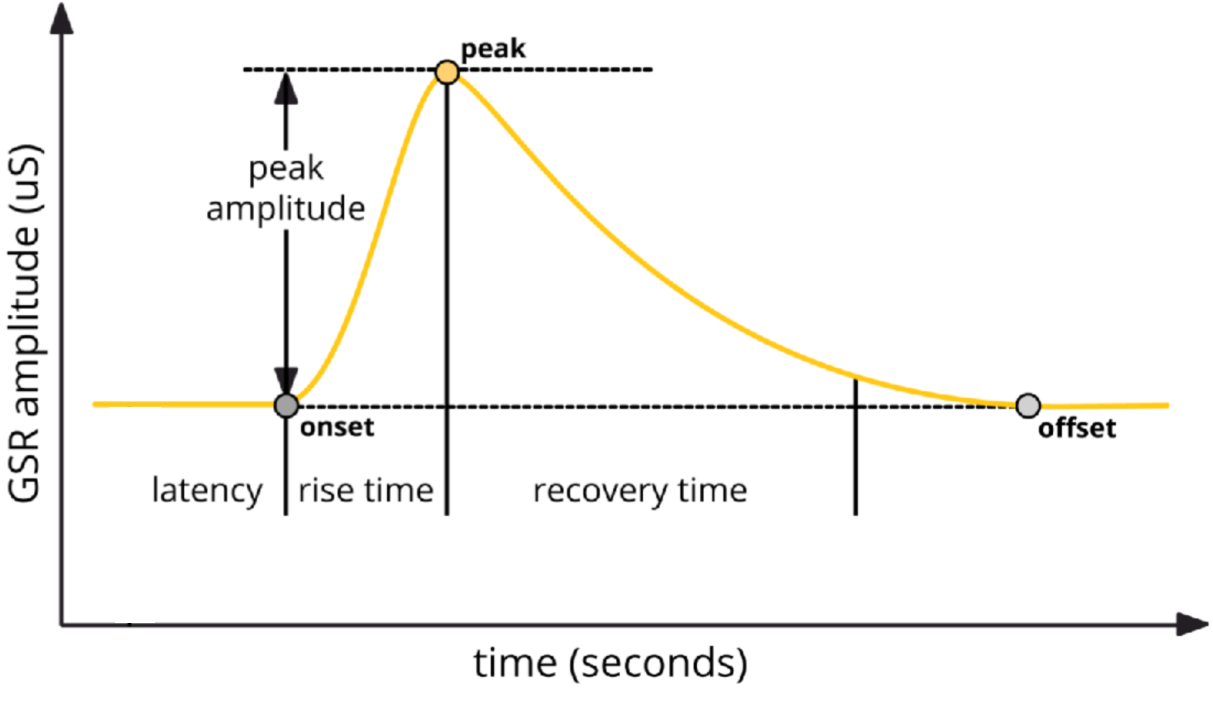
\includegraphics[width=11cm]{Images/peaks.png}}
\caption[Spitzenz{\"a}hler-Merkmal]{Spitzenz{\"a}hler-Merkmal: Onset (Startpunkt), Spitze und Offset (Endpunkt). Jedes Paar von Onset/Offset erh{\"o}ht die Anzahl der Spitzen um eins.} 
\label{fig:peaks} \end{figure} \vspace{0.5cm}


Jedes handgefertigte Merkmal wird auf einem Zeitfenster von Daten f{\"u}r jeden Sensorkanal unabh{\"a}ngig voneinander angewendet. 
Jedes Zeitfenster ist daher 117 Merkmalen zugeordnet (9 Sensorkan{\"a}le multipliziert mit 13 Merkmalen). \\





% Unterkapitel 
\subsubsection{Codebook Approach} \label{ca-1}


Die bisherige Methodik mit handgefertigten Merkmalen ist klassisch f{\"u}r den {\"u}berwachten Lernansatz. 
Es existieren aber auch einige Nachteile. 
Das Hauptproblem besteht darin, dass nicht sichergestellt werden kann, dass die gew{\"a}hlten Merkmale die besten Klassifizierungsergebnisse erzielen. Damit besteht immer die Gefahr, dass m{\"o}glicherweise andere Merkmalen bessere Ergebnisse liefern w{\"u}rden, diese handgefertigten Merkmale aber die  nicht gefunden wurden. Dieses Risiko besteht insbesondere bei der physiologischen Signalverarbeitung zur Emotionserkennung, wo die Struktur der Daten noch recht unbekannt und allgemein komplex ist. 
Eine weitere Schwierigkeit besteht darin, relevante selbstentwickelte Features ohne Expertenwissen {\"u}ber die Daten zu finden.
Dar{\"u}ber hinaus wurden noch keine gut funktionierenden State-of-the-Art handgefertigten Merkmale identifiziert.
Aus diesen Gr{\"u}nden ist es interessant halbautomatische und un{\"u}berwachter Ans{\"a}tze der Merkmalsextraktion zu verwenden und zu testen. \\


K. Shirahama et al. \cite{kimiaki_codebook_approach_2016} schlugen eine un{\"u}berwachte Merkmalsextraktionsmethode namens Codebook Approach (CA) vor, um Merkmale aus 1D-Zeitreihensignalen zu erzeugen.
Der CA hat den Vorteil, dass formbasierte Merkmale gefunden werden k{\"o}nnen, die f{\"u}r das Problem der Emotionserkennung relevant sind, aber weder offensichtlich noch leicht als Mensch zu interpretieren sind. 
Der CA besteht aus drei Schritten, die in den folgenden Abschnitten erl{\"a}utert werden: Codebuchkonstruktion (engl. "codebook construction"), Codewortzuordnung (engl. "codeword assignment") und der anschlie{\ss}enden Klassifizierung. \\


\textbf{Codebuchkonstruktion \\}
Ziel dieses Schrittes ist es, Teilsequenzen (sogenannte "Codew{\"o}rter") zu bestimmen, die f{\"u}r die 1D-Eingangssensorik charakteristisch sind. 
Dies wird erreicht, indem Zeitfenster aus dem urspr{\"u}nglichen Datensatz f{\"u}r jeden Sensorkanal unabh{\"a}ngig voneinander nach dem im Kapitel \ref{segmenation-1} definierten Segmentierungsansatz extrahiert werden.
Aus jedem so erhaltenen Zeitfenster der Gr{\"o}{\ss}e $T$ werden kleinere Segmente der Gr{\"o}{\ss}e $\alpha$ unterteilt.
Ein Clustering-Algorithmus wird dann auf die Menge der Segmente $\alpha$ angewendet, um Clusterzentren zu finden.
Nach der Konvergenz werden die Clusterzentren als Codew{\"o}rter betrachtet und zum Aufbau einer Sammlung von Codew{\"o}rtern mit dem Namen ``Codebuch'' verwendet, wie in Abbildung \ref{fig:ca_construction} aus \cite{kimiaki_codebook_approach_2016} dargestellt. 
Die Anzahl der Codew{\"o}rter (d.h. die Gr{\"o}{\ss}e des Codebuchs oder die Anzahl der Cluster) ist ein Hyperparameter des Verfahrens. Im Rahmen dieser Arbeit wurde ein k-means Clustering-Algorithmus verwendet, um die Codew{\"o}rter auf den ELISE-Daten zu erhalten. \\


\begin{figure}[h]\centering{
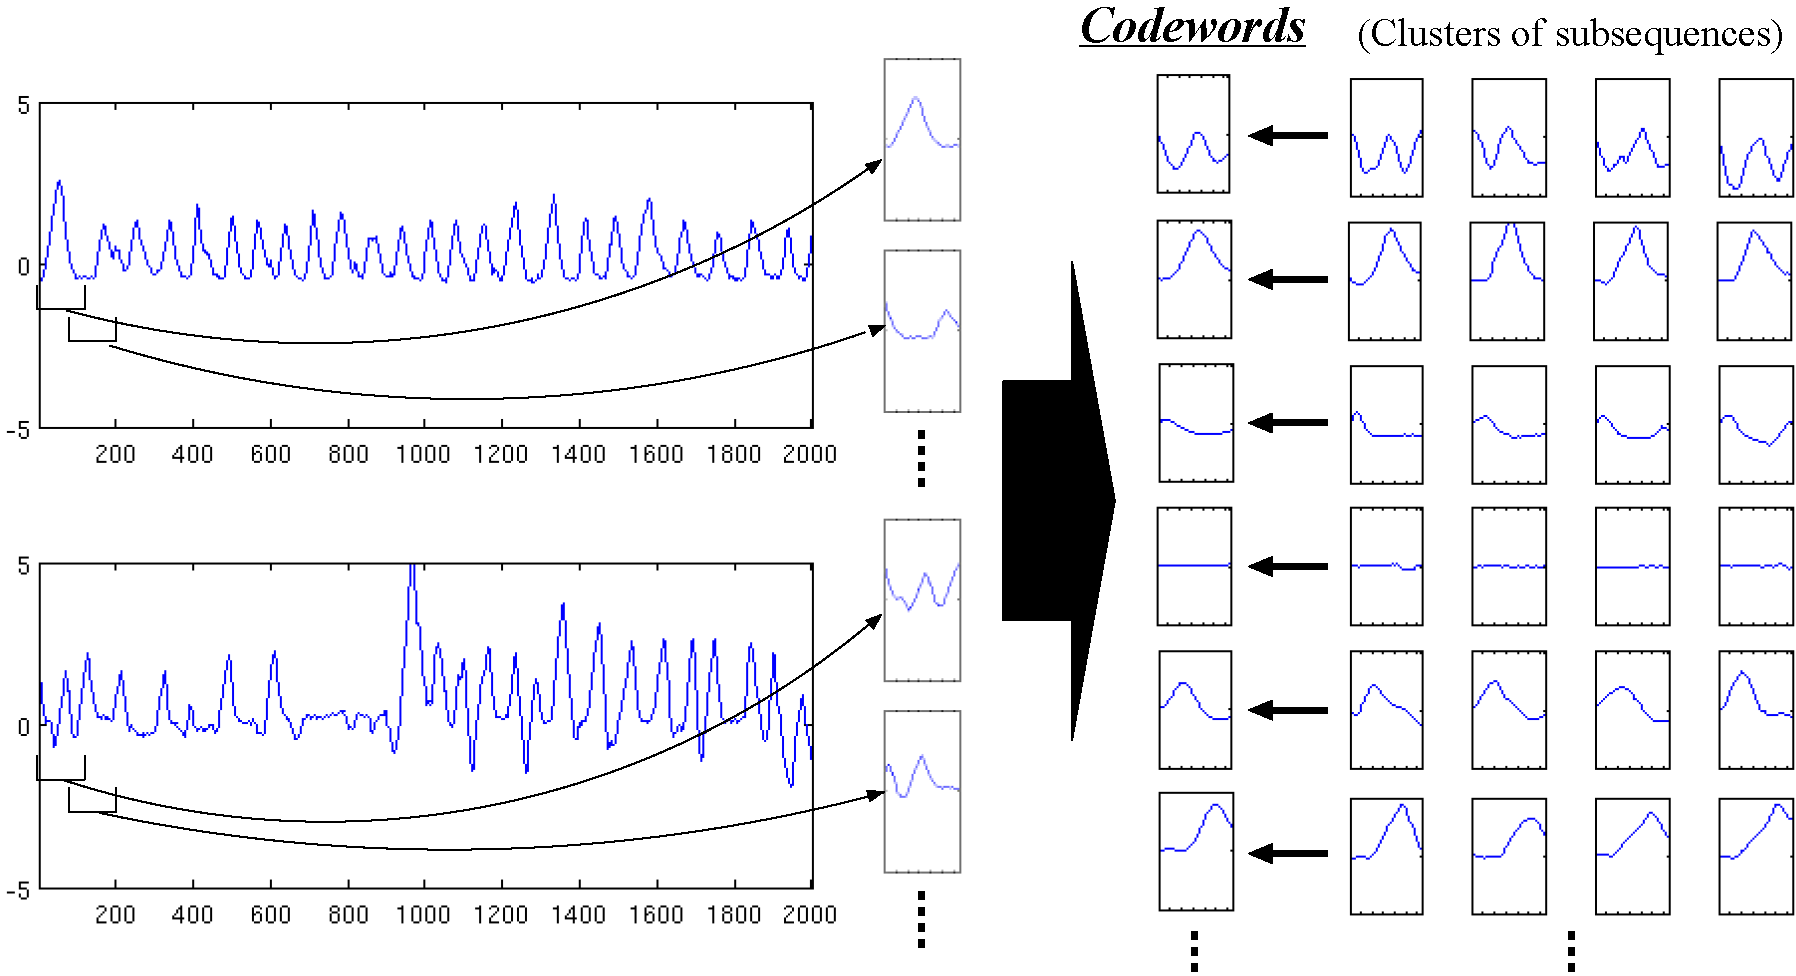
\includegraphics[width=\textwidth]{Images/CA_construction.png}}
\caption[Codebuchkonstruktion]{Codebuchkonstruktion: Zeitfenster von Daten werden zun{\"a}chst extrahiert. Ein Clustering-Algorithmus wird dann auf das alle Zeitfenster angewendet, um Clusterzentren (und damit Codew{\"o}rter) zu finden, die zum Aufbau des Codebuchs verwendet werden. }
\label{fig:ca_construction} \end{figure} \vspace{0.5cm}


\textbf{Codewortzuordnung \\}
Nach der Konstruktion der Codew{\"o}rter wird f{\"u}r jedes Zeitfenster $T$ ein histogrammbasierter Merkmalsvektor erstellt (vgl. Abbildung \ref{fig:ca_assignment}, entnommen aus \cite{kimiaki_codebook_approach_2016}). 
Der zu klassifizierende Datensatz wird zun{\"a}chst in Zeitfenster der Gr{\"o}{\ss}e $T$ segmentiert, aus denen Segmente der Gr{\"o}{\ss}e $\alpha$ nach dem gleichen Verfahren wie beim Aufbau des Codebuchs extrahiert werden. 
Jedes Segment $\alpha$ wird dann mit den Codew{\"o}rtern verglichen, so dass das "{\"a}hnlichste" Codewort gefunden werden kann. 
Ein K-Bin-Histogramm (mit $K$ Anzahl der Codew{\"o}rter) mit Informationen {\"u}ber die Anzahl der Male enth{\"a}lt, die jedes Codewort als am {\"a}hnlichsten zu den Segmenten $\alpha$ im Zeitfenster $T$ betrachtet wurde, wird dann erstellt und als Merkmalsvektor verwendet, um das zu klassifizierende Zeitfenster $T$ darzustellen. 
Das Ma{\ss} f{\"u}r die {\"a}hnlichkeit von Codew{\"o}rtern und Datensegmenten $\alpha$ basiert auf der euklidischen Entfernung. \\


\begin{figure}[h]\centering{
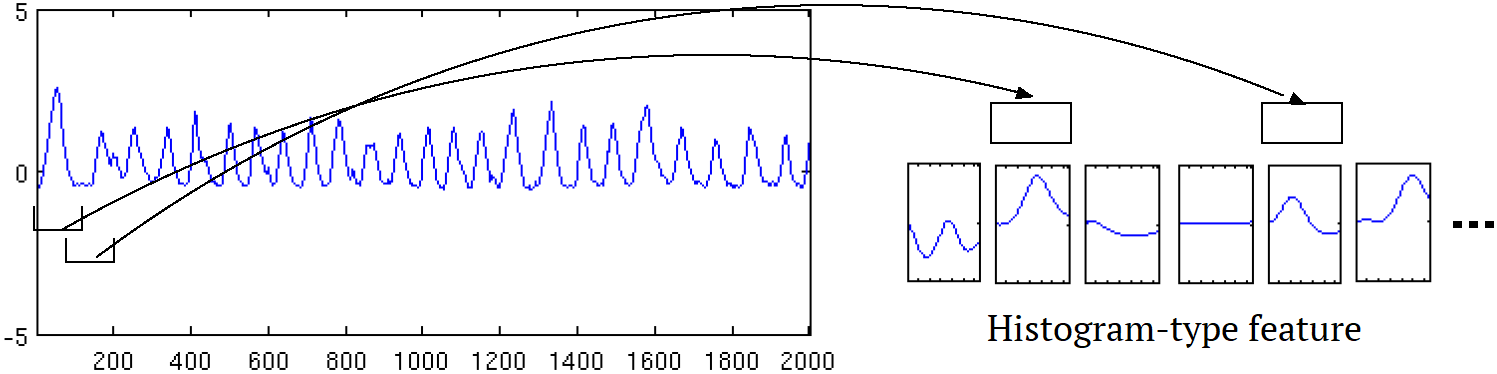
\includegraphics[width=\textwidth]{Images/CA_assignment.png}}
\caption[Codewortzuweisung]{Codewortzuweisung: Jedes Datensegment wird mit den Codew{\"o}rtern verglichen und ein Histogramm mit Informationen dar{\"u}ber, wie oft jedes Codewort als "am {\"a}hnlichsten" betrachtet wurde, wird erstellt. }
\label{fig:ca_assignment} \end{figure} \vspace{0.5cm}


Der zuvor beschriebene Ansatz wird als "Hard-Zuordnung" (engl. "hard assignment") bezeichnet, da Datensegmente einem einzigen Codewort zuzuordnen werden.
Ein Nachteil dieser Vorgehensweise ist die mangelnde Flexibilit{\"a}t im Umgang mit potenzieller Unsicherheit bei der Codewortzuweisung, die z.B. auftreten kann, wenn ein Zeitfenster von Daten zwei oder mehr Codew{\"o}rtern sehr {\"a}hnlich ist, da es nur einem zugeordnet werden kann. 
Ein alternativer Ansatz dieses Problem zu umgehen ist die so genannte "Soft-Zuordnung" (engl. "soft assignment"). Hierbei werden auch alle Codew{\"o}rter des Codebuchs Datensegmenten zuzuordnen, wobei die {\"a}hnlichkeit jeweils als ein Bin im Histogramms dargestellt wird. Sehr {\"a}hnlich entspricht hierbei einem hohen Wert und nicht {\"a}hnlich einem kleinen Wert (anstatt 0 oder 1 wie in der Variante der Hard-Zuordnung). 
Eine Kerneldichtefunktion (vgl. \cite{gemert_ieee_2009}) wird verwedent, um die Histogramm-Bins zu berechnen. Es wurde die folgende Funktion verwendet:


\begin{equation} 
\Large{ {f(\alpha,c_k,p) = \frac{1}{\gamma}} \frac{g(\alpha,c_k,p)}{\sum_{i=1}^{K} g(\alpha,c_i,p)}}
\end{equation}
\newline
wobei $f(\alpha,c_k,p)$ die {\"a}hnlichkeit des Segments $\alpha$ bezeichnet, das sich auf das Codewort $c_k$ bezieht. $p$ ist ein Gl{\"a}ttungsparameter (ein gro{\ss}es $p$ bewirkt eine starke Gl{\"a}ttung), $\gamma$ ist die Anzahl der Segmente im Zeitfenster $T$ und: \\
\begin{equation} 
\Large{ { g(\alpha,c_k,p) = \frac{1}{\sqrt{2 \pi p^{ 2 }}}} exp(\frac{d(\alpha,c_k)}{2p^{2}}). }
\label{equ:codeword_assignment_2} \end{equation}
\newline
Um numerischen Unterlauf zu vermeiden, wird die Gleichung (\ref{equ:codeword_assignment_2}) zun{\"a}chst mit dem Log-Sum-Exp-Trick (vgl. \cite{murphy_2012}) berechnet. \\




\textbf{Fusion mehrerer Sensoren \\}
Oftmals werden mehrere Sensoren verwendet, die gleichzeitig mehrere verschiedene Signale derselben Emotion erzeugen.
Die Fusion dieser Signale ist wichtig, da sie die Genauigkeit der Emotionserkennung verbessern kann.
Es gibt zwei verschiedene Ans{\"a}tze (vgl. \cite{snoek_2005}): die fr{\"u}he Fusion (engl. "early fusion") und die sp{\"a}te Fusion (engl. "late fusion"): 

\begin{itemize}
  \item \underline{Fr{\"u}he Fusion:} In der Dimension $K \times S$ wird nur ein Klassifizierer ben{\"o}tigt, wobei $K$ die Anzahl der Codew{\"o}rter und $S$ die Anzahl der Sensorkan{\"a}le ist. Der Klassifikator wird anhand der Verkettung von Codebuchmerkmalen trainiert und ausgewertet, die auf jedem Sensorkanal unabh{\"a}ngig voneinander berechnet wurden.

  \item \underline{Sp{\"a}te Fusion:} Erfordert mindestens $S$-Klassifikatoren (einen f{\"u}r jeden Sensorkanal). Ein Klassifizierer wird unabh{\"a}ngig f{\"u}r jeden Sensorkanal unter Verwendung der f{\"u}r den betrachteten Sensor erhaltenen Codebuchmerkmale trainiert. Die Vorhersagen der $S$-Klassifikatoren werden dann fusioniert, um die Klassenbezeichnung des zu klassifizierenden Zeitfensters zu sch{\"a}tzen (z.B. mit einem zus{\"a}tzlichen Klassifizierer).
\end{itemize} \vspace{0.5cm}


In dem ELISE Projekt verwenden wir den sp{\"a}ten Fusionsansatz, weil er rechnerisch g{\"u}nstiger ist und von K. Shirahama (vgl. \cite{kimiaki_codebook_approach_2016}) empfohlen wird. \\













% Unterkapitel 
\subsubsection{Deep Neural Networks (DNN)} \label{dnn-1}
Im Rahmen des ELISE Projektes, wurden verschiedene Deep Neural Networks (DNN) getestet\cite{bscschnieber18}.
Die Standardarchitektur Multilayer Preceptron (MLP), Long Short-Term Memory Network (LSTM), ein CNN/LSTM Hybrid, eigene MLP-Architekturen sowie multimodale MLP (vgl. Abbildung \ref{fig:multimodal_dnn} und multimodale CNN wurden bewertet.
Alle Ansätze erhalten Datenfenster der Größe $T \times S$ als Input, mit $T = 420$ aufgenommene Datenpunkte pro Sekunde jedes Sensors und $S = 9$ Sensorkanäle. 
Jedes Modell hat einen Softmax-Output-Layer mit vier Neuronen, jeweils einen pro Klasse.
Da die Softmax-Funktion monoton ist und die Summe aller Ergebnisse immer eins ergibt, ist jedes einzelne Ergebnis auch gleichzeitig die Wahrscheinlichkeit, dass the aktuelle Input zu einer Klasse gehört.
Alle Modelle wurden mit einem ADADELTA-Optimierer\cite{zeiler12} trainiert, wobei die entsprechenden Hyperparameter (z.B. Anzahl der Layer, Neutronen pro Layer, ...) manuel ausgewählt wurden. \\

Der verwendete MLP hat drei zusätzliche verstecke Layer mit 1.000 Neutronen und ReLU-Aktivierung\cite{nair12}.
Alle Layer sind verbunden, d.h. der Output aller Neutronen eines Layers werden als Input eines jeden einzelnen Neutronen auf den nächsten Layer. \\



\begin{figure}[H]\centering{
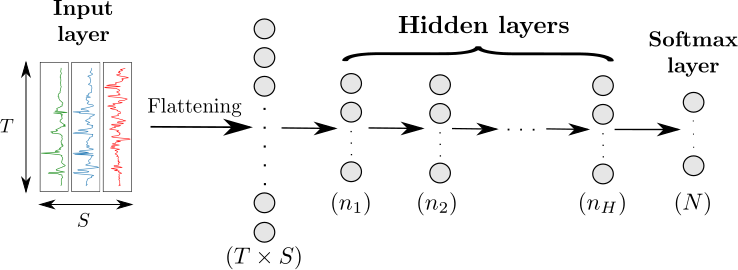
\includegraphics[width=\textwidth]{Images/mlp.png}}
\caption{Architektur eines MLP Network. }
\label{fig:mlp} \end{figure} \vspace{0.5cm}



Die verwendete CNN besteht aus drei faltungsbedingten Layern mit zehn Filter-Kernels und jeweils einem ReLU.
Die Kernel-Größe ist $41 \times 1$ for den ersten Layer, $21 \times 1$ für den zweiten und $11 \times 1$ für den dritten Layer.
Da die zweite Dimension immer eins ist, funktioniert jeder Kernel immer nur an einem Sensorkanal.
Alle faltungsbedingten Layer werden gefolgt von einem Maxpooling-Layer der Größe $2 \times 1$, welcher den Output um den Faktor zwei downsamplet. \\


\begin{figure}[H]\centering{
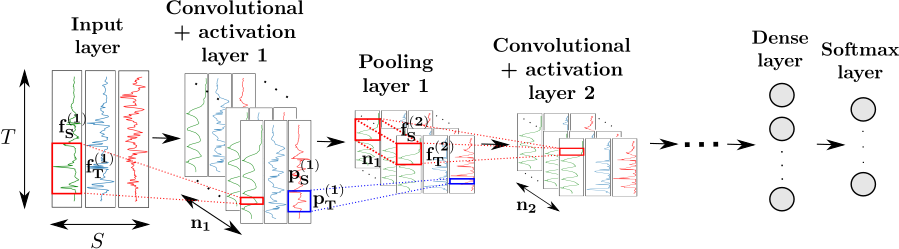
\includegraphics[width=\textwidth]{Images/cnn.png}}
\caption{Architektur eines CNN Network. }
\label{fig:cnn} \end{figure} \vspace{0.5cm}



Für MLP und CNN wurde zusätzlich ein Multimodal-Network getestet, welche auch bekannt als mMLP bzw. mCNN sind.
Anstatt das ganze Zeitfenster als Input zu benutzen, wird hier jeweils ein Neural-Network mit drei versteckten Layern für jeden Sensorkanal verwendet (siehe Abbildung \ref{fig:multimodal_dnn}).
Die Ergebnisse wurden zusammengeknüpft und als Input für ein zusätzlichen verbindeten Layer genutzt. \\


\begin{figure}[H]\centering{
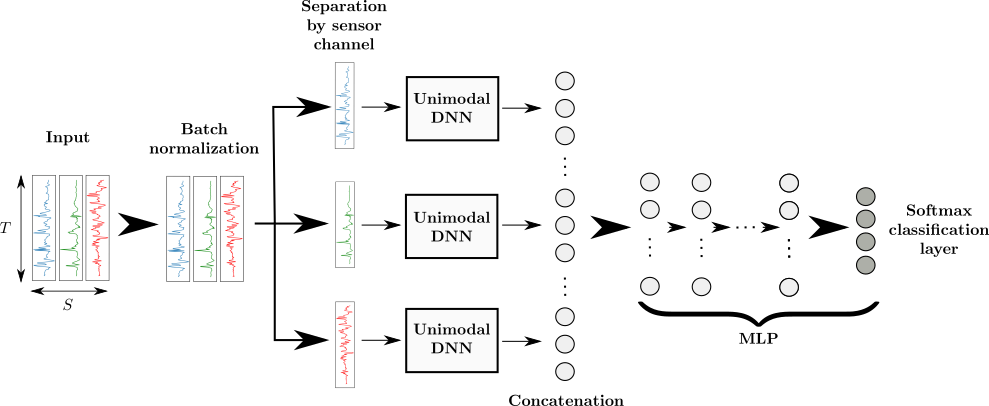
\includegraphics[width=\textwidth]{Images/multimodal_dnn.png}}
\caption{Eigene Architektur eines Multimodal-MLP-Network. }
\label{fig:multimodal_dnn} \end{figure} \vspace{0.5cm}


LSTMs\cite{hochreiter97} sind eine spezielle Form von wiederkehrenden Neural-Networks.
Sie sind in der Lage, Informationen zu speichern, um Muster über die Zeit zu erkennen. 
Nicht wiederkehrende Neural-Networks lernen im Gegensatz dazu nur von den aktuellen Input-Daten.
Das Verhalten über die Zeit gesehen wird von den sogenannten ``Gates'' kontrolliert, welche den Informationsfluß innerhalb eines Networks beeinflußen können.
Das ``Input-Gate'' sakralisiert den Einfluss des neuen Daten-Inputs, während das ``Forget Date'' den Einfluss der gespeicherten Informationen über den vorherigen Zustand des Neurons steuert.
Am Ende wird der neue Output von dem ``Output-Gate'' modifiziert. \\


\begin{figure}[H]\centering{
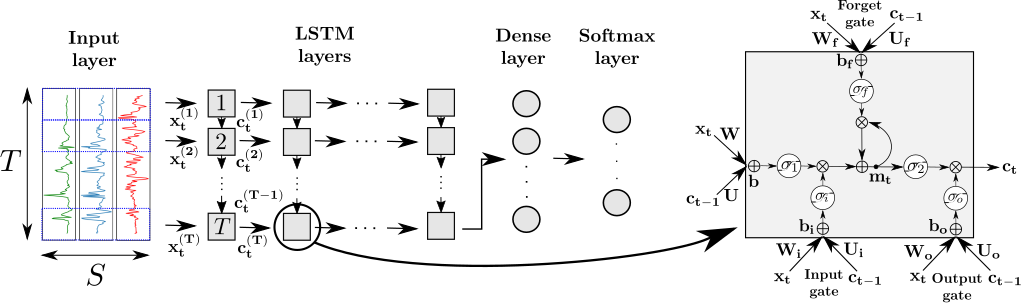
\includegraphics[width=\textwidth]{Images/lstm.png}}
\caption{Architektur eines LSTM-Networks. }
\label{fig:lstm} \end{figure} \vspace{0.5cm}


Das CNN/LSTM-Hybrid-Modell stapelt einfach die beiden Networks.
Die ersten Layer sind die der vorhin geschriebenen CNN, welche dann von den Layern der LSTM-Layer gefolgt werden. \\


\begin{figure}[H]\centering{
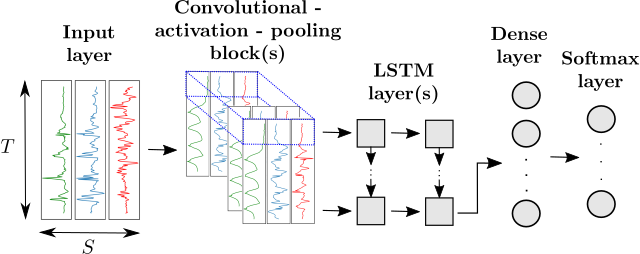
\includegraphics[width=\textwidth]{Images/cnn_lstm.png}}
\caption{Architektur eines CNN/LSTM-Hybriden. }
\label{fig:cnn_lstm} \end{figure} \vspace{0.5cm}














% Unterkapitel 
\subsubsection{Merkmals Auswahl} \label{featureSelection-1}

Um bessere Kombinationen von handgefertigten Merkmalen zu finden, kann ein Bottom-Up-Merkmal-Auswahlalgorithmus verwendet werden, der auf der Pr{\"u}fung von Gruppen von Merkmalen mit zunehmender Gr{\"o}{\ss}e basiert.
Zun{\"a}chst wird das Merkmal mit der h{\"o}chsten Klassifizierungsperformance unter allen verf{\"u}gbaren Merkmalen ausgew{\"a}hlt. 
Anschlie{\ss}end wird die Performance von Gruppen von zwei Merkmalen, die sich aus dem ausgew{\"a}hlten Merkmal und der Reihe nach jedem anderem Merkmal zusammensetzen, werden dann getestet und das beste Paar wird ausgew{\"a}hlt. 
Dieser Prozess wird so lange wiederholt wiederholt, bis alle relevanten Merkmale verwendet wurden. 
Am Ende wird die beste Kombination von Merkmalen ausgew{\"a}hlt.
Es sei darauf hingewiesen, dass es sich um einen heuristischen Algorithmus handelt, so dass es m{\"o}glich ist, dass unter Umst{\"a}nden die absolut beste Kombination nicht zwingend gefunden wird. \\

Der folgende Pseudocode beschreibt unseren Algorithmus zur Merkmalsauswahl: \\

\begin{algorithm}[H]
    \SetKwInOut{Input}{Input}
    \SetKwInOut{Output}{Output}
    
    %\vspace{0.1cm}

    %\underline{function feature-selection} $(features, C, kernel, \gamma)$\;
    
    \textbf{Input parameters:}  \\
    \hspace{0.5cm} - $C$, $\gamma$ = C-SVM params \\
    \hspace{0.5cm} - $candidates$ = $[f1,f2,...,fn]$ list of n features to test \\
    \hspace{0.5cm} - $training\_set$ = set of all features computed on the training data \\
    \hspace{0.5cm} - $testing\_set$ = set of all features computed on the testing data 
    %\vspace{0.1cm}
    
    \textbf{Output parameters:} \\
    \hspace{0.5cm} - $best\_feature\_combination$ = list of the best features \\
    \hspace{0.5cm} - $best\_accuracy$ = classification accuracy obtained by the best features \\
    \hspace{0.5cm} - $feature\_ranking$ = list ranking features in decreasing order of relevance
    %\vspace{0.1cm}
    
    \hrulefill 
    
    %\vspace{0.1cm}
    %\textbf{Pseudo-code:} \\
    \textbf{Begin} \\
    $candidates\_to\_test$ = $candidates$ \\
    $current\_best\_features$ = $\emptyset$ \\
    $current\_best\_accuracy$ = -1 \\
    $all\_time\_best\_features$ = $\emptyset$ \\ 
    $all\_time\_best\_accuracy$ = -1 \\
    $feature\_ranking$ = $\emptyset$ 

     \While{$candidates\_to\_test \neq \emptyset$}{
         \For{$feature f$ \textbf{in} $candidates\_to\_test$}{
             $trained\_svm$ = $train\_svm(C, \gamma, training\_set, current\_best\_features \cup \{f\}$) \\
             $accuracy$ = $evaluate\_svm(trained\_svm, testing\_set, current\_best\_features \cup \{f\}$)
        
             \If{$accuracy > current\_best\_accuracy$}{
                 $best\_feature\_of\_iteration$ = $f$ \\
                 $current\_best\_accuracy$ = $accuracy$
            }
                
             \If{$accuracy > all\_time\_best\_accuracy$}{
                 $all\_time\_best\_features$ = $current\_best\_features \cup \{f\}$ \\
                $all\_time\_best\_accuracy$ = $accuracy$ 
            }
        }
         $feature\_ranking$ = $feature\_ranking \cup [best\_feature\_of\_iteration]$ \\
         $current\_best\_features$ = $current\_best\_features \cup [best\_feature\_of\_iteration]$ \\
        $candidates\_to\_test$ = $candidates\_to\_test \setminus [best\_feature\_of\_iteration]$ \\
    }
     \textbf{return} $all\_time\_best\_features, all\_time\_best\_accuracy, feature\_ranking$
    

    %\vspace{0.3cm}
    \caption{ Merkmalsauswahl-Algorithmus. }
\end{algorithm}
\vspace{0.5cm}